\begin{savequote}[75mm] 
La verdad no penetra en un entendimiento rebelde. Si todos los lugares de la tierra est\'{a}n en el Aleph, ah\'{i} estar\'{a}n todas las luminarias, todas las l\'{a}mparas, todos los veneros de luz.
\qauthor{Jorge Luis Borges, El Aleph} 
\end{savequote}

\chapter{Integration of Information in Bioinformatics} \label{section:integration}


\begin{description}
	\item[First author publications]:\\
		\begin{enumerate}
			\item \label{paper:mydas} \bibentry{SAL2012}
			\item \label{paper:writeback}\bibentry{SAL2011}
			\item \label{paper:msctheses}\bibentry{SAL2010}
		\end{enumerate}
 	\item[Coauthor publications]:\\
		\begin{enumerate}
			\setcounter{enumi}{3}
			\item \label{paper:dasty3} \bibentry{VIL2011}
%			\item \label{paper:mykaryoview} \bibentry{JIM2011}
		\end{enumerate}

	\item[Author's Contibutions]:\\
		\begin{itemize}
			\item \emph{\ref{paper:mydas}}: Conceived and designed the experiments: GS. Performed the experiments: GS AJ. Wrote the paper: GA LG PJ RJ. Critical revision of the manuscript for important intellectual input: RJ AQ AJ NM MM SH HH. Technical and material support: AJ NM MM SH HH. Supervision: NM MM SH HH. Study concept: GS LG PJ AQ RJ HH. Architectural design: PJ GS. Software development: GS LG PJ AQ. Evaluation of the compatibility with DAS protocol: AJ.
			\item \emph{\ref{paper:writeback}}: Critical revision of the manuscript for important intellectual input: RJ, AG, HH, NM and EB. Technical and material support: HH, NM and EB. Study supervision: HH, NM and EB. Study concept: GS, RJ and AG. Architectural design: GS and EB. Software development: GS. Drafting of the manuscript: GS. Design of the usability experiment: GS, NM and EB. All authors read and approved the final manuscript.
			\item \emph{\ref{paper:msctheses}}: MSc theses by GS, Supervision by EB, Co-supervision by NM
			\item \emph{\ref{paper:dasty3}}: Critical revision of the manuscript for important intellectual input: JV, RJ LG,GS, BG, NM, MM, AG and HH. Technical and material support: HH, NM, AG and MM. Study supervision: HH, NM, AG and MM. Study concept:  RJ and HH. Architectural design: JV, GS, BG and RJ. Software development: JV. Drafting of the manuscript: JV, AG and LG. All authors read and approved the final manuscript.
%			\item \emph{\ref{paper:mykaryoview}}: Conceived and designed the experiments: RCJ MC NM JD. Performed the experiments: RCJ MC. Analyzed the data: MC. Contributed reagents/materials/analysis tools: GS BG. Wrote the paper: MC.
		\end{itemize}
\end{description}
\newpage

\newthought{The data analysed in bioinformatics comes from diverse and heterogeneous sources}, for example, the data might be captured from wet-lab experiments or deduced from \emph{in-silico} procedures. It can refer to nucleic acid information and sequenced data, but also to expression levels and other protein related information. It is possible to analyse isolated organisms or to gather information from multiple species. It all depends on the purpose of the research and the availability of data, however it is almost inevitable to have to integrate more than one of these sources in order to tackle today's research challenges.

This chapter is focused on the contributions made during this PhD to the integration of data using the Distributed Annotation System. The first section describes  MyDas, a server tool that facilitates the publishing of DAS sources. A proposal to extend DAS in order to support collaborative annotation is described in section \ref{section:writeback}. We have grouped our participation in several client-side projects with DAS into section \ref{section:dasvisual}. Lastly we discuss the impact of these projects, together with the present and future status of DAS. 

\section{MyDas} \label{section:mydas}

The research in this section has been published in the paper \cite{SAL2012}, referenced as \ref{paper:mydas}, at the beginning of this chapter. Authors of this paper are Gustavo A. Salazar, Leyla J. García and Philip Jones (first authors). The co-authors provided input in line with their roles as supervisors.  Parts of this section are based on the work of collaborators and this is indicated clearly below. 

The contributions to the software development process of MyDas are as follows: the first version of the project was developed by Philip Jones with the collaboration of Anthony Quinn for the XSLT component. A second development cycle together with the support of the DAS version 1.6 was executed by Gustavo A. Salazar. Current maintenance of the software is led by Leyla J. García. As an open source project, it has received contributions from other developers, but the authors mentioned here have been the leaders of the project during its various stages.

\subsection{Overview}

As of January 2015, there were over 1500 sources registered in the DAS registry, and although not all of them implement the same capabilities, they all follow the DAS protocol with almost half of them updated to the latest version DAS 1.6E. There are common tasks among DAS sources:  parsing, capture of arguments, exception handling, XML creation, dealing with the HTTP protocol, and more. Therefore, software specialised in these tasks is needed in order to allow data providers to focus on their specific cases.

MyDas is a software tool that assists in the process of publishing biological data through the DAS protocol, described in \ref{ssec:DASprotocol}. Data providers are required to implement an adaptor that connects the logic of MyDas with the data itself, and from there MyDas executes all the HTTP interfaces, XML encodings and other required operations to support all the DAS capabilities.

In the following sections we describe the architecture of MyDas, and present some examples of existing DAS services built upon MyDas.

\subsection{ Design and Implementation}
MyDas is a Java Servlet Application which accepts HTTP requests, typically with one request for each command in the DAS specification. Responses are valid XML documents. MyDas is a Java 1.6 application, and it runs on a Java servlet container such as Tomcat (\url{http://tomcat.apache.org/}) or Jetty (\url{http://jetty.codehaus.org/jetty/}). 

Figure \ref{fig:mydas} illustrates the architecture of MyDas, which is clearly divided between core and external control. The MyDas core is in charge of all the common tasks and the external control is what needs to be input by the data provider, for instance its storage system (e.g. a relational database or flat file), or the strategy used to query the data (e.g. in-memory or using pre-indexing), etc.

The development process of MyDas is supported by several tools, for example, it uses Maven (\url{http://maven.apache.org/}) for automatising the software built, control of dependencies, test and deployment. It also uses JUnit (\url{http://www.junit.org}) to create a set of unit tests to ensure the quality of the software. Software workers are implemented on the repository machine to execute the tests when new commits are submitted which notifies the main developers in case of failure.

\begin{figure}[t]
\centering
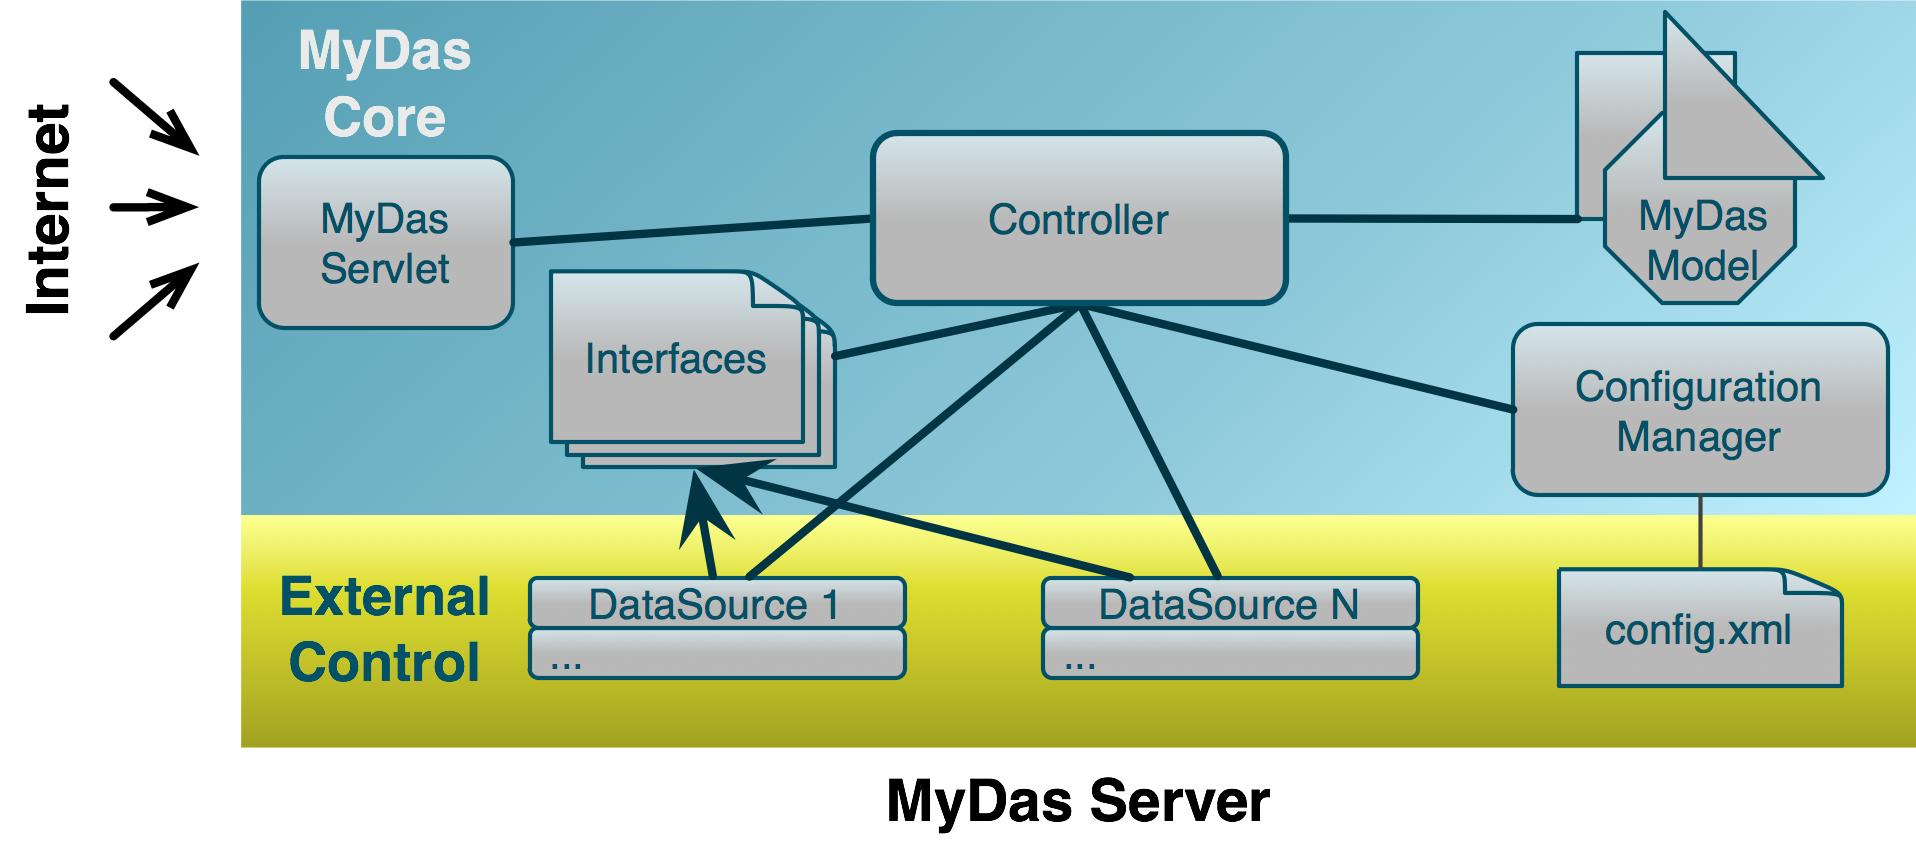
\includegraphics[width=\textwidth]{figures/MydasArchitecture.png}
\caption[MyDas Architecture.] {MyDas Architecture. The requesters can interact with MyDas through the servlet, which communicates the commands to the Controller. The Controller knows which Data Sources have been implemented by querying the Configuration Manager. Data Sources should implement at least one of the provided Interfaces. MyDas internally implements the DAS model.
\label{fig:mydas}}
\end{figure}

The information required to use the external control components should be described in the configuration file, including data such as the URI, title and the relative path to the data source adapter. Then, the configuration manager makes the user options available to both the MyDas core and the data source implementation. 

The elements of the DAS specification have been mapped into a Java object model, which must be used by the data source developer when creating an adapter. In this way , the core of MyDas can use the same subroutines to deploy heterogeneous data into DAS. 

In order to facilitate the implementation of data sources, a template project is available with examples of both reference and annotation servers: \url{https://code.google.com/p/mydas/downloads/detail?name=MyDasTemplate-1.6.7.zip}.

\subsection{Instances}
MyDas is being adopted by different data providers, including UniProt, InterPro and PRIDE.

UniProt (Universal Protein Resource)\cite{UNI2011} is a comprehensive catalogue of protein sequences and functional information. It consists of different databases, each optimized for different uses. The UniProt Knowledgebase (UniProtKB) is an expertly curated database providing a central access point for integrated protein sequence information. The UniProt Archive (UniParc) is a non-redundant sequence repository of all publicly available protein sequences. UniProt DAS (\url{http://www.ebi.ac.uk/das-srv/uniprot/das/uniprot}, \url{http://www.ebi.ac.uk/das-srv/uniprot/das/uniparc}) acts as a reference and annotation server, providing access to up-to-date information and allowing queries by UniProtKB and UniParc accessions numbers. There are currently more than 50 Data Sources that use UniProt DAS as a reference.

The InterPro database of predictive protein signatures is used for the classification and automatic annotation of proteins and genomes \cite{HUN2009}. InterPro provides several DAS data sources: DS\_327 (\url{http://www.ebi.ac.uk/das-srv/interpro/das/InterPro} ) serves matches that have been calculated to the predictive models supplied by the InterPro member databases for all UniProtKB protein sequences.  DS\_1028 (\url{http://www.ebi.ac.uk/das-srv/interpro/das/InterPro-matches-overview}) serves these matches resolved to the InterPro entries that integrate the member database signatures (providing a compact summary view of the domains, families and sites predicted for each UniProtKB sequence). Finally DS\_1029 (\url{http://www.ebi.ac.uk/das-srv/interpro/das/InterPro-UniParc-matches}) serves matches to member database signatures that have been calculated for UniParc protein sequences.

PRIDE DAS 1.6 (\url{http://www.ebi.ac.uk/pride-das/das/}) provides protein and peptide identifications together with supporting mass spectrometry evidence \cite{VIZ2009}. The information from PRIDE has already been shared using BioMart\cite{KIN2011}, therefore the strategy used to make it public to the DAS community was to develop an adaptor using MyDas to take the information from this source.

\subsection{Tutorials}
We have developed three tutorials on how to use MyDas that are accessible via the web (\url{http://code.google.com/p/mydas/wiki/Tutorials}). The tutorials are classified by their level of difficulty: Beginner, Intermediate and Advanced. 

The first tutorial helps the user in the setup of the example data source. No programming is required at this point, as it is limited to installation and configuration of MyDas. The intermediate level tutorial guides the user through the common scenario of having a text file with some annotations that need to be displayed in DAS. In this case, the user is required to program the parsing of the file and mapping of it into the model. The third tutorial explores the case of obtaining data from a database system, which is a common way to store/access data in bioinformatics environments. This tutorial requires not only the ability to program in Java, but also to understand queries written in SQL.

The power of MyDas is revealed when it is used on large data sets with elaborate schemas as in the last tutorial. The example uses the freely available mysql database provided by Ensembl. There are over a hundred databases hosted on the Ensembl servers, and in this case we used the core set of tables for Homo Sapiens (version 56\_37a), and restricted our search scope to some high level features (e.g. Chromosome, genes, transcript). 

Many institutions may have a similar setup, however schema, policies and software vary from one location to another. Although exporting files (and using them to publish data) is an option, it implies that changes in the database won't be reflected in the generated files. In contrast, MyDas can be set up to take the information directly from the database management system and therefore will always be up to date.

\begin{figure}[t]
\centering
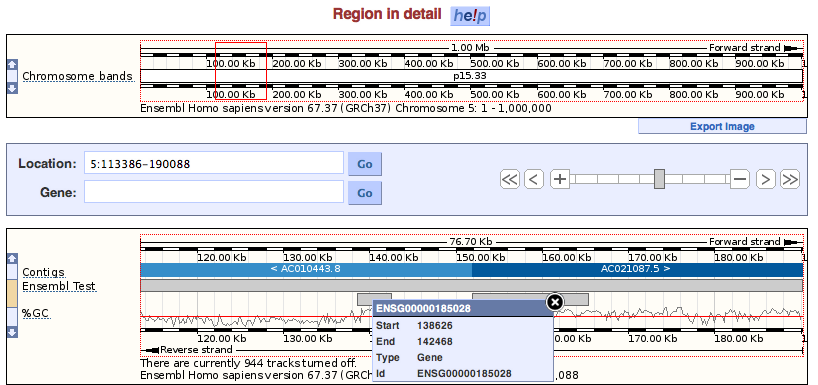
\includegraphics[width=\textwidth]{figures/MyDasEnsembl.png}
\caption[A MyDas Source as displayed on the Ensembl client.] {The data source created during the MyDas tutorials as it is visualised on the Ensembl web browser.
\label{fig:mydas_example}}
\end{figure}

A data source served by MyDas can be used by several tools to visualize its data. Figure \ref{fig:mydas_example} is a snapshot of the Ensembl browser, including the track named `Ensembl Test', whose information is obtained from the tutorial data source. This demonstrates how the data published with MyDas can be displayed in well known genome browsers.

\subsection{Other DAS Servers}
The second tutorial mentioned above, describes the case where a user has a plain text file that follows a basic format (i.e. separated by a predefined character). This scenario is so common in bioinformatics that a software tool specialising in the publishing of this type of data has been built. easyDAS\cite{GEL2011}  is a preinstalled server where a new data source can be configured by submitting a GFF file (or similar). This alternative is ideal for rapid publishing because it simplifies the tasks related to the hosting and storage of both data and server. The drawback is the lack of control over the data once it is deployed, because the owner of the data won't be able to change individual values of a dataset that has been submitted, instead, he would be required to delete and upload the whole data source.

\begin{table}[t]
        \begin{tabular}{| l | l | l | l | l |}
\hline \rowcolor{table_header}
\emph{Feature} & \emph{MyDas} & \emph{ProServer} & \emph{Dazzle} & \emph{easyDAS}\\
\hline \rowcolor{row_odd}
Language & Java & Perl & Java & Web App(Perl)\\
\hline \rowcolor{row_even}
Latest Release & 2011 & 2011 & 2010 & 2011\\
\hline \rowcolor{row_odd}
DAS Version & 1.6 & 1.6 & 1.53E\footnotemark  & 1.6\\
\hline \rowcolor{row_even}
Physical Storage & Defined by User & Defined by User & Defined by User & Internal database\\
\hline \rowcolor{row_odd}
Entity Responsible & EBI & Sanger Institute & Sanger Institute & EBI\\
\hline \rowcolor{row_even}
Create a data source & Develop Java class & Develop Perl adaptor & Develop ava class & Submit a tab-file\\
\hline \rowcolor{row_odd}
        \end{tabular}
        \caption{Features of the main DAS servers}
        \label{tab:table1}
\end{table}
\footnotetext{There is a branch of this project where the capabilities of DAS 1.6  have been implemented, however there was not a stable version of it at the time of publishing.}

Besides MyDas, there are other implementations of DAS servers such as Dazzle (\url{www.biojava.org/wiki/Dazzle}) or ProServer \cite{FIN2007},  amongst others (see \url{http://www.biodas.org/wiki/DAS/1#Implementation}). Nonetheless, MyDas and ProServer are the only servers that fully support the current DAS specification (1.6E). They differ from each other mainly in the language in which they are implemented (ProServer is written in Perl), but not in feature set, making system compatibility the major factor in deciding between the two.

Table \ref{tab:table1} summarizes some of the high level characteristics of the most well known DAS servers.


Some benchmarking tests were executed in order to compare  MyDas, ProServer and Dazzle and evaluate their loading performance. The tests were run with the Apache HTTP Server Benchmarking Tool (\url{http://httpd.apache.org/docs/2.0/programs/ab.html}).  easyDAS was not considered for this test because it is installed on a different server, therefore there is no way to exclude network latency from the test.

The three servers were installed on the same machine, and data sources with the same data set were created on each. We prepared three DAS queries with expected responses of approximately 1.5Kb, 200Kb and 7.5Mb. Each query was repeated 1000 times with 10 concurrent connections

The 3 servers were able to complete all the requests and table \ref{tab:table2} shows the main results of the executed test.

\begin{table}[!ht]
        \begin{tabular}{| l | l | l | l |}
\hline \rowcolor{table_header}
\emph{Figure} & \emph{MyDas} & \emph{ProServer} & \emph{Dazzle}\\
\hline \rowcolor{row_odd}
Requests per Second - Mean (small) & 739.88 & 1.54 & 424.56\\
\hline \rowcolor{row_even}
Time per request - Mean (small) & 13.516 ms & 6492.978 ms & 23.554 ms\\
\hline \rowcolor{row_odd}
Transfer Rate (small) & 1534.68 Kbytes/sec & 2.81 Kbytes/sec & 859.91 Kbytes/sec\\
\hline \rowcolor{row_even}
Requests per Second - Mean (medium) & 51.52 & 1.40 & 34.10\\
\hline \rowcolor{row_odd}
Time per request - Mean (medium) & 194.114 ms & 7123.396 & 293.216 ms\\
\hline \rowcolor{row_even}
Transfer Rate (medium) & 10944.96 Kbytes/sec & 288.19 Kbytes/sec & 6997.52 Kbytes/sec\\
\hline \rowcolor{row_odd}
Requests per Second - Mean (large) & 1.79 & 0.32 & 1.10\\
\hline \rowcolor{row_even}
Time per request - Mean (large) & 5589.148 ms & 30942.590 ms & 9110.292 ms\\
\hline \rowcolor{row_odd}
Transfer Rate (large) & 13088.38 Kbytes/sec & 2283.04 Kbytes/sec & 7770.29 Kbytes/sec\\
\hline \rowcolor{row_even}
        \end{tabular}
        \caption{Benchmarking between the main DAS servers.}
        \label{tab:table2}
\end{table}

This comparison can not be considered conclusive in deciding which is the best or fastest DAS server, mainly because each data source has unique challenges and different cases can generate different results. Nonetheless, given that the three servers provide a data source implementation to publish data from a GFF file, they were configured to use the same GFF file to ensure equal conditions. 

The figures in the table show that in all three scenarios MyDas performed better than the other servers. It is important to note that both MyDas and Dazzle were running on the same Tomcat server, therefore the conditions for both were the same. ProServer on the other hand, is a standalone server that implements socket communications in the application itself, which is an advantage in terms of making it easy to use.

The complete results of the tests are available in Appendix \ref{ap:stress}.








\section{DAS Writeback}\label{section:writeback}

A large part of the work included in this section was carried out prior to the timeframe of this PhD during the MSc referenced as No. \ref{paper:msctheses} at the beginning of this chapter. Nonetheless, the inclusion of this contribution in this document is relevant because the software was reengineered as part of this PhD, upgrading it to the latest DAS specification and using the most recent versions of its dependencies: MyDas and DASty3. The results of both the MSc and reengineering process were published in the article \ref{paper:writeback} as reported at the beginning of this chapter. The first author of the paper is Gustavo A. Salazar and the co-authors provided input in line with their roles as collaborators and supervisors. 

\subsection{Overview}
DAS offers a uniform protocol to share data that can, and has, been used by diverse data providers. One of the advantages of this approach is that users can now  collect information from multiple resources by using a single tool. However we consider that opening the communication in the opposite direction (i.e. users submitting annotations to the resources), is a desirable functionality that was not included in the first versions of the protocol.

For example, researchers using a DAS client to gather information about a protein of their interest can identify errors in existing features or missing annotations. It is unrealistic to expect such a user to deploy a new DAS source to publish a handful of annotations. The traditional alternative is for them to report the new features to the providers. This however takes time, and has the inconveniences associated with using a centralised repository (as mentioned in section \ref{subsec:dwh}), where the user might have to wait for the release of a new version of the data before it can actually be used in the client.

As a solution to this problem, we have designed and implemented the Distributed Annotation System (DAS) Writeback, which enables community-based manual annotation of public data. Our approach makes the process of manual annotation a collaborative task, whereby any individual can participate by sharing their knowledge in the form of new or edited annotations.

The DAS Writeback system provides the capabilities of reading, writing, editing and deleting features by users of a web application. For the design and development of such a system it was necessary to model an architecture that supports the new features, define an extension of the DAS specification to accommodate the client-server communication, and implement server and client components. All of these milestones were achieved while trying to follow the same style as the existing DAS technology,with the object of achieving easy adoption of the system by the DAS community.

\subsection{DAS as RESTful services}
The strategy used to define the architecture of a writeback system for DAS was to reconcile two technical concepts: on the one hand, DAS uses the REST protocol for web services \cite{PRL2007}, and on the other hand, reading and writing functionalities have been widely explored in Relational DataBase Management Systems (RDBMS), where the basic operations are  known as CRUD (Create, Read, Update and Delete) \cite{KIL1990}.

One of the major strengths of the RESTful strategy is that it is based on such widely adopted standards as HTTP, XML, URI and MIME. This makes REST, and therefore DAS, technologies easy to implement and attractive to both developers and end users. Considering this we decided that when extending the DAS protocol to support servers that can store edited annotations, we set out to retain compatibility with the existing read-only system of HTTP GET requests. 

One of the main features of the REST architecture is to have a uniform interface. This means that REST resources should be manipulated using a predefined set of operations. In the case of the Web, those operations are the 4 basic reading/writing operations CRUD, and the HTTP methods PUT, GET, POST and DELETE are suggested in the literature to specify those actions. These operations \textit{``are broadly applicable but they also help uphold specific Web architectural properties''} \cite{VIN2008}.

Version 1.53E of the DAS specification includes a detailed explanation of the reading and querying capabilities of the system. This however only covers the use of GET, and there is no mention of any of the other RESTful methods.

Our proposal was to extend the DAS protocol in order to define the use of the other RESTful methods to complete the inclusion of the CRUD functionalities into the DAS system, and consequently, provide the DAS community with appropriate tools for collaborative annotation.

A previous effort in a similar direction was the object of a MSc thesis, where a DAS Writeback server was developed as a proof of concept \cite{GRZ2008}, however it used different technologies and wasn't closely attached to the RESTful protocol, which are factors that we consider to be key in the adoption of any extension on DAS.

\subsection{Architecture}
The components of the system were developed bearing the following goals in mind:

\begin{enumerate}
\setlength\itemsep{-0.5em}
\item The original annotations of a DAS source should not be modified directly.
\item The system should be trusted by the user.
\item The system should promote interaction between the server and users.
\end{enumerate}

The first goal has been established in order to ensure that the data shared by a provider is not at risk of being changed or deleted through any case of vandalism or by mistake when using the write back system. In order to do this, the architecture includes a third party writeback server that stores the changes to a set of annotations, independent of the original source providing those annotations. 

New features, edits and deletions are saved on the writeback server as annotations themselves and therefore they can in turn be edited or deleted by other users. We hope that this feature gives the users the sense of trust (goal 2) that other collaborative systems such wiki projects have, where the community ensures the quality of the information. 

Finally, as a means to promote the use of the writeback system, we implemented its functionalities in the well known protein DAS client: DASty. The purpose of this was to introduce the writeback functions to an existing interface that users were already familiar with.

\begin{figure}[ht] 
\centering
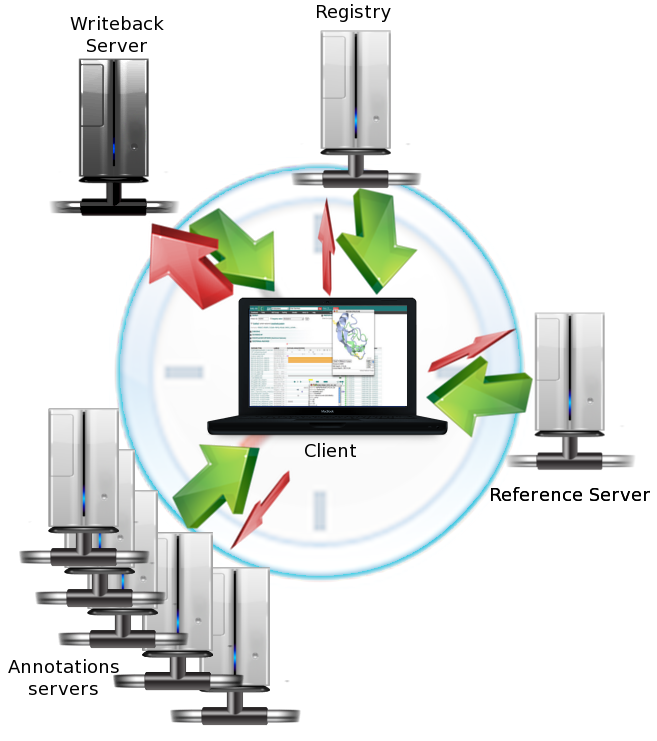
\includegraphics[width=4in]{figures/WritebackArchitecture.png} 
\caption[Writeback in the DAS Architecture]{\emph{Writeback in the DAS Architecture}: Extension of the DAS architecture for the writeback. A third party writeback server is the last to be queried by the client, and its response is used to update the information provided by the annotation servers. Communication with the writeback server has the peculiarity that the amount of information sent by the client is considerably larger than for any other server. The clock in the background represents the chronological order of the actions in a DAS transaction.}  \label{fig: WritebackArchitecture}
\end{figure}

Figure \ref{fig: WritebackArchitecture} represents the architecture of DAS including the writeback server. Firstly it is necessary to highlight that, when a feature is requested, the writeback server behaves as another annotation server, using the same DAS commands. The way this information is rendered is the responsibility of the client. 

A standard DAS transaction starts by querying the DAS Registry (the DAS Registry provides a repository for the registration and discovery of DAS services). Next the reference sequence is obtained, followed by parallel requests to several annotation sources. The interaction between client and writeback occurs after the client has retrieved and displayed all of the information for the target protein, since it is only then that the user has a complete landscape view to take the decision to add, update or delete a feature.

HTTP requests relating to write operations on the writeback server are much larger than standard DAS requests (shown in Figure \ref{fig: WritebackArchitecture} as the width of the red arrow). The reason for this is that the client is now required to send the information to add or update a specific feature, including its type, category, position and other characteristics predefined in DAS. The communication with the writeback server is thus extended beyond the display of a graphic that compiles the information from all the servers. This is when the user starts to interact with the information, transforming the client from a pure visualisation tool to an interactive interface between the user and the DAS data.

\subsection{Protocol Extension}
As described in \ref{ssec:DASprotocol}, version 1.53 of the DAS protocol was expanded in version 1.53E, where a set of proposed extensions were included. The same schema was followed when version 1.6 was released, shortly followed by 1.6E, when it was decided by the DAS community that new extensions could be proposed using the wiki page of the project (\url{http://www.biodas.org}). Their adoption by the community would determine their inclusion as a core component in future versions.

We followed these guidelines in order to include the writeback into DAS, which eventually became the first official extension of DAS 1.6E. The specification can be found on the DAS1.6E web page (\url{http://www.biodas.org/wiki/DAS1.6E\#DAS\_writeback}). It indicates that both input and output documents for the writeback should follow the DAS GFF format (See code below for an example). The HTTP method determines what to do with the received document; the GET method is still being used for querying and reading; while POST, PUT and DELETE should be used to create, update or delete features respectively.

The HTTP status codes used for DAS remain valid and indicate success or failure of the requested command (e.g. HTTP code 200 for success)

%\newpage
\begin{lstlisting}
<?xml version="1.0" standalone="no"?>
<DASGFF>
 <GFF>
    <SEGMENT id="P13569" start="1" stop="1480" version="f29b8c0a9056a0f7680f3290d259b6ac">
       <FEATURE id="new" label="ISFCSQFSWIMPGTIK">
           <TYPE id="Polypeptide" cvId="Polypeptide">Polypeptide</TYPE>
           <METHOD id="ECO:0000160" cvId="ECO:0000160">
                   Inferred from protein separation followed by fragment identification
           </METHOD>
           <START>488</START>
           <END>503</END>
           <NOTE>note added in the writeback</NOTE>
           <NOTE>USER=username</NOTE>
           <NOTE>PASSWORD=password</NOTE>
       </FEATURE>
    </SEGMENT>
 </GFF>
</DASGFF>
\end{lstlisting}


\subsection{Implementation}
We have developed a DAS writeback tool by extending existing DAS clients and servers. The writeback is included as a plug-in of DASty3 and is integrated in the latest implementation of MyDAS. It is also compliant with the current DAS 1.6 specification. 

\subsubsection{Server}
Our implementation of DAS Writeback is an extension of the MyDAS server, which has been widely described in section \ref{section:mydas}. A writeback data source was implemented to store annotations. Annotations are the main entity in the data model, and any edits or deletions of an annotation are considered to be versions of the original annotation.

The datasource uses Hibernate \cite{BAU2006} as its layer to access the persistence data, which brings the advantage of being \emph{Database-Engine} independent. The data source has been successfully tested using PostgreSQL, MySQL and Derby; but is expected to work in other engines.

\subsubsection{Client}\label{section:dastywb}
One of the goals of this project was to create the perception for users that the writeback functions in a client are native and can be used naturally with existing clients. For this reason, the extension of an existing client was preferable to implementing a new one from scratch. In addition, the writeback server behaves as any other DAS server for reading purposes, so many software routines of an existing client could potentially be reused for the writeback visualisation.

We decided to use DASty for our first DAS writeback client and a prototype was developed for DASty2, which is detailed in \cite{SAL2010}. We collaborated in the development of some of the components of DASty2 \cite{JIM2008} and our knowledge of the software influenced the decision to use it for the writeback.

Later, in 2010, DASty2 went through a refactoring process, optimising its code to provide a plug-in framework. The new version is called DASty3 and our contribution to its development is described in section \ref{section:dasty}. The writeback client was rewritten as a plugin for DASty3 and is included in its core feature set.


\subsubsection{CRUD functions}
Below we describe how the CRUD functions (i.e. Create, Read, Update, Delete) have been implemented in both client (DASty3 plugin) and server (MyDas extension).

\begin{figure}[ht]
\centering
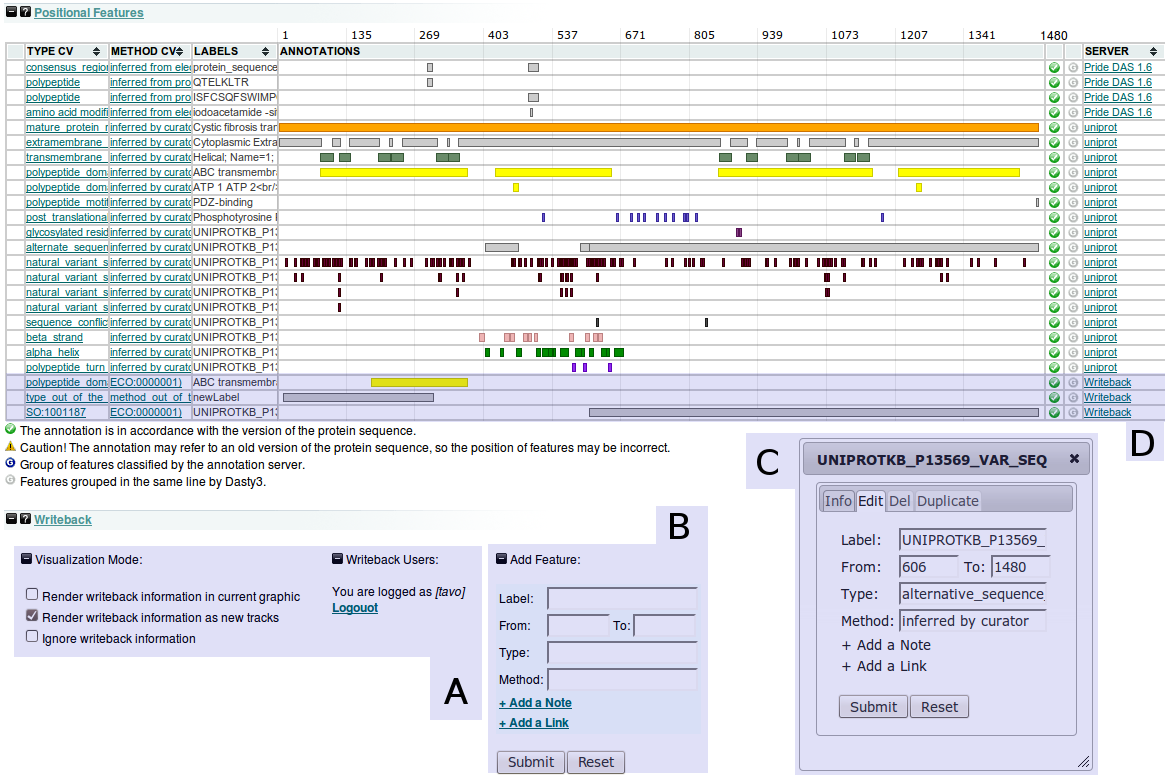
\includegraphics[width=6.5in]{figures/dasty3wbT.png} 
\caption[Writeback extensions on DASty3.]{Writeback extensions on DASty3. (A) Modes to visualize the informations from a writeback server into the DASty3 features graphic. (B) Form to add a new feature. (C) popup window including writeback related tabs, for edit, deletion and duplication of features. (D) Annotations from the writeback server displayed in the features panel.  
\label{fig: dasty+wb}}
\end{figure}

\paragraph{Create}
Previous versions of MyDas used GET and POST methods interchangeably, therefore the first modification of the server was to identify the different HTTP methods and redirect the flow of data to its corresponding action. In order to create a new annotation, MyDas now listens to activity from any POST method, and if its content is a GFF file, it is parsed and added to the data source. 

On the client side, a new form was added under the annotation graphic (\ref{fig: dasty+wb} B) in which the user can describe the new feature specifying label, location, type and evidence. Notes and links are optional fields for the new feature. 

Version 1.6 of the DAS specification recommends the use of ontologies in order to standardise both annotation type and evidence codes, and make the task of integrating annotation from several servers easier. In order to promote the use of those ontologies, a list of suggested terms from the corresponding ontology is displayed in the edit form.
  
\paragraph{Read}
The writeback server behaves like any other DAS source when a set of features is requested. The client decides when and how to process this information. For the DASty3 writeback plug-in, the user has three different modes to choose from (Figure \ref{fig: dasty+wb} A): (i) to ignore the writeback annotations, (ii) to use the writeback as any other annotation source, or (iii) to replace original annotations with the writeback information. The latter option generates a similar graphic for features as normally rendered by DASty3, but incorporating the modifications that the writeback server contains. 

\paragraph{Update}
When a DASty3 user clicks on a feature, a popup window with the complete information of the annotation is displayed. We have extended this functionality by including tabs on the popup window. The ``Edit'' tab contains a similar form to that of a new feature, but it is filled with the information of the selected annotation (Figure \ref{fig: dasty+wb} C). 

The information of this form is sent to the server using the method PUT. MyDas identifies the method, parses the GFF document and stores its content as the current version of the feature. The latest version will be the one to which the server returns for future requests.

\paragraph{Delete}
Del is another tab available in DASty3 when a feature is selected. Its content is just a confirmation dialog where the user expresses the desire to remove that feature. The DELETE HTTP method is then invoked, including the feature's identifier. When MyDas detects a DELETE requests, it creates another annotation to register this command.  This means that features are not really deleted from the server. Rather, the features tagged as deleted will be transparent in the DASty3 graphic, and only its border will be visible.


\subsubsection{Other writeback functions}
A basic module to allow for user authentication through a login and password was added in the writeback panel (Figure \ref{fig: dasty+wb} A). Any writing function is conditional on prior login and password validation. The reading functionality does not require authentication.

Another way to edit a feature is through the history tab. In this window, the content of any previous version of the selected feature is displayed. The user can choose to roll-back to a previous version, which submits a new edit request through the PUT HTTP method. Therefore a roll-back task does not remove the existing history, but rather adds a new edit to it.



	
\section{DAS Clients} \label{section:dasvisual}
The architecture of the Distributed Annotation System described in \ref{ssec:DAS} passes a large part of the responsibility of integrating data to the client, whose job is simplified by the fact that all the sources comply with a protocol. Although DAS is mostly associated with the integration of information, DAS clients have been developing visualisation strategies in order to provide a single view of the collected information.

In the following subsections we will describe our contributions to two DAS clients: DASty and probeSearcher. Through these projects, we have observed the power of integrating information using web based visualisation techniques. Users can visit the website of any of these tools wherever they are, and through the DAS client get information from multiple sources. This information can then be condensed into a single view, which can be explored further in order to get more detailed information.

\subsection{DASty} \label{section:dasty}
Our first contribution to the DAS technology was in 2008, when we assisted in the development of a component for DASty2 which included the visualization of the 3D structure of a protein in parallel with its annotations, allowing the user to highlight the coverage of a feature in its structure. Later, as part of this PhD we collaborated on the reengineering of this software. The results of this collaboration are described in \cite{VIL2011} and are also referenced at the beginning of this chapter as the co-author publication No. \ref{paper:dasty3}. Our contribution to the development of the software was focused on the software design and definition of the architecture. Implementation, documentation and maintenance were tasks executed by our collaborators. 

DASty was originally developed using Macromedia Flash for the client and Java for the server component. It included the basic functionalities of an annotation viewer (e.g.  alignment of annotations against the protein sequence, manipulation of the graphic) and was strongly attached to the UniProt DAS source \cite{JON2005}. 

The project was re-written in 2007 to take advantage of the novel features offered at the time by a technology known as Asynchronous Javascript And XML (AJAX). There are three main advantages of using AJAX for a DAS client:
\begin{enumerate}
\item The possibility of having asynchronous calls to a server allows the client to generate responses on-the-fly, and in this way the user can analyse partial results of fast servers, while slow ones take their time to reply.
\item The DAS specification uses XML to define the responses of a DAS server, and AJAX was designed to use XML for the same purposes. Therefore routines in the AJAX API can be reused for the processing of well-formed XML documents, such as the ones defined using the DASGFF format.
\item AJAX is part of Javascript and is therefore supported by all the main browsers. Besides that, the processed XML response can be used to manipulate the HTML rendered in the webpage. The whole system uses the technologies that are natively implemented in web browsers, and therefore there is no need for any third party libraries (e.g. Flash, Java.).
\end{enumerate}

The interface of DASty2 organises its available functionalities as interconnected panels. In the \emph{search panel}, the user can include the accession number of a protein of interest and select groups of DAS sources to search. Once the search starts, multiple information messages are included in the \emph{status panel}, and a progress bar indicates how many servers have responded. The first response to be displayed comes from the reference server, including the sequence of the protein which is then rendered in the \emph{sequence panel}. The \emph{positional features panel} contains the protein annotation browser, which gets updated by each response of an annotation source. These responses also include information that relates to the whole protein and not only to a part of it, which in DAS terminology are known as non-positional features. These features are grouped and displayed in the \emph{non-positional features panel}. All these results can be filtered by type, server name and evidence code by using hierarchical lists that are displayed in the \emph{filtering panel}. A last request is invoked to check if the protein has 3D structures reported in the PDB database. If this is the case, the user can select one and it will be displayed in the \emph{protein structure panel} \cite{JIM2011}.

In the DASty3 project we re-engineered the software to not only offer the same range of capabilities as DASty2 but to also provide ``\emph{a framework upon which tools can be built and integrated into a cohesive web environment}'' \cite{VIL2011}. We defined a modular architecture (Figure \ref{fig:dasty-architecture}), which supports the extension of DASty3's functionality by using plugins and templates.

\begin{figure}[ht]
\centering
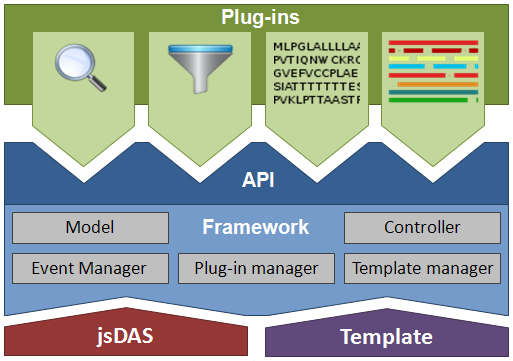
\includegraphics[width=4.5in]{figures/dasty3_architecture.png} 
\caption{DASty3 Architecture}  \label{fig:dasty-architecture}
\end{figure}

DASty3 templates allow the definition of styles through CSS, but more importantly, it supports manipulation of the complete interface through Javascript. This feature provides a way to adapt DASty3 to different environments, for example, if an institution decides to embed DASty3 into a web application, they can personalise the DAS client to not only follow the fonts and colours of the institution, but also to follow the same web layout of the application.

New features and visualisations can be included in DASty3 with the implementation of plugins. We defined a rich API that developers can use to interact with the different components of DASty3. For instance the interaction between plugins is done by implementing the broadcaster--listener metaphor using standardised events that can be used (to trigger or to listen) by any of the components in DASty3

All the communication between DASty3 and the different DAS entities is handled with jsDAS(\url{https://code.google.com/p/jsdas/}), a Javascript library that supports the DAS commands and parses the sources' responses into a data structure. This model is reused inside the DASty3 core and its plugins.

\begin{figure}
\centering
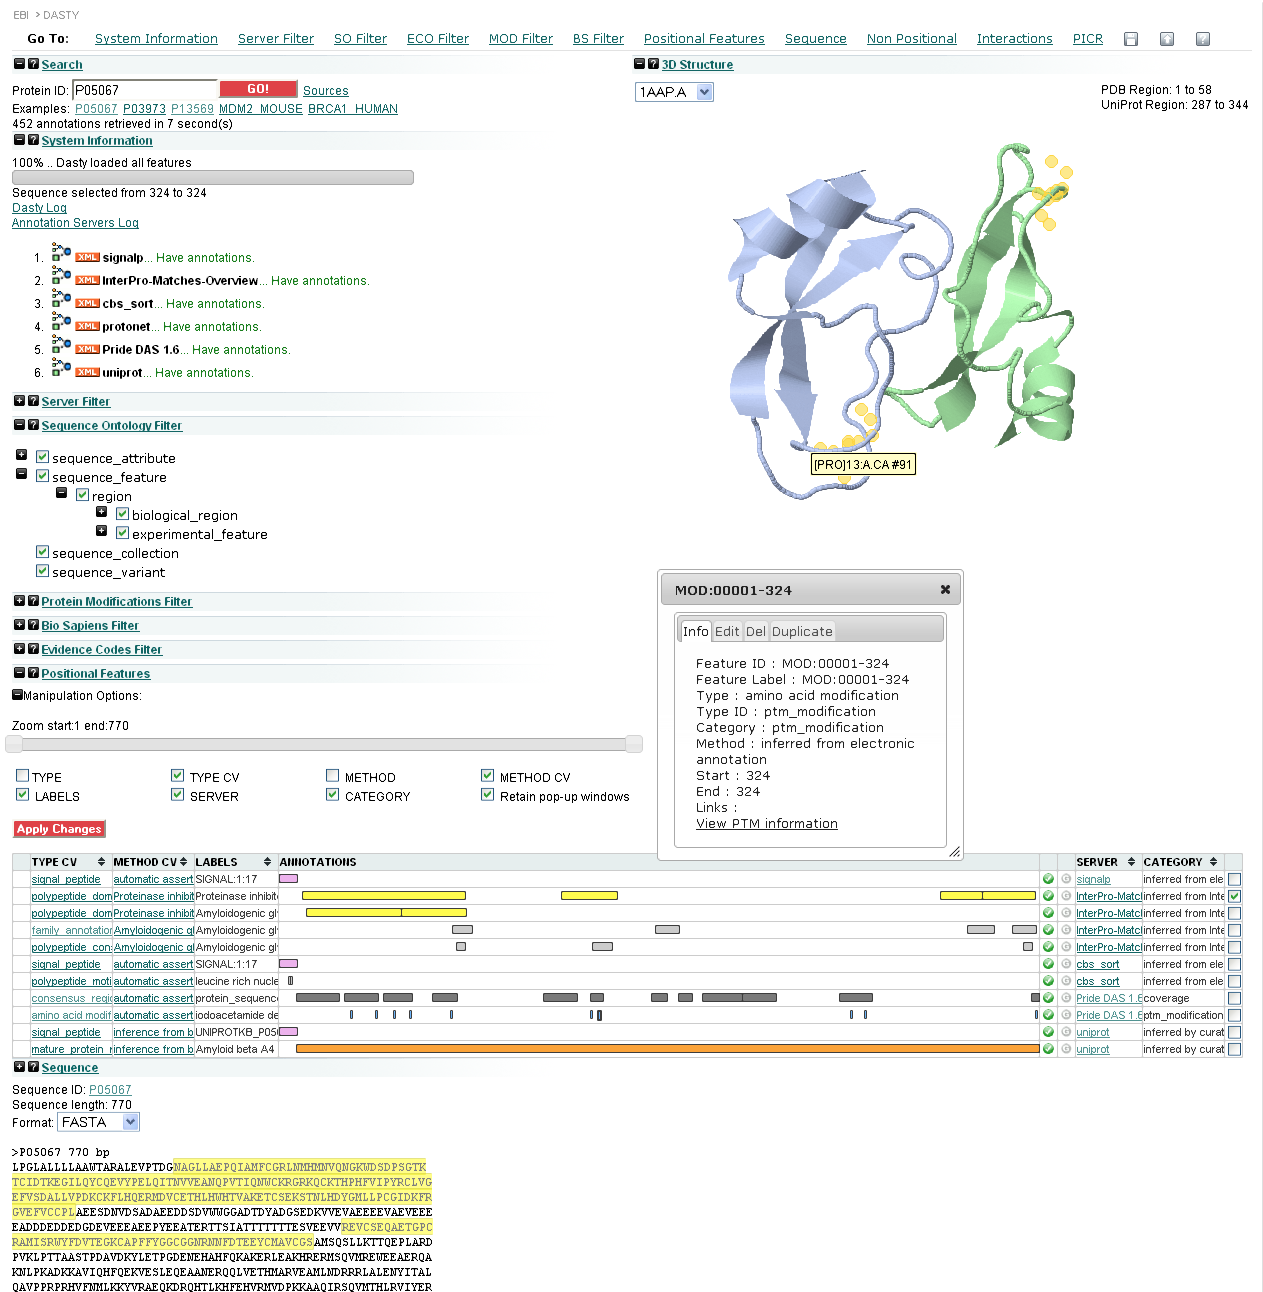
\includegraphics[width=\textwidth]{figures/dasty3.png} 
\caption{Snapshot of DASty3}  \label{fig:dasty3}
\end{figure}


Figure \ref{fig:dasty3} is a snapshot of DASty3, in which it is possible to identify the different panels that were mentioned above for DASty2. We decided to keep a similar "look and feel" for the application to facilitate its adoption by regular users of DASty2. 

Figure \ref{fig:dasty3} also illustrates the communication between plugins. When a user selects a track on the annotation browser (see the checkbox at the right side of the second track), an event notifying this action is fired, and several plugins react accordingly. For instance, the sequence plugin highlights the amino acids covered by the features on the track using the same colour as in the graphic, and simultaneously the 3D structure plugin highlights the corresponding parts in the current PDB file.

\subsubsection{Writeback plugin}
While developing the writeback plugin for DASty3 described in section \ref{section:dastywb}, several software contributions were made to DASty3. Besides bug fixes and minor changes, there were a few significant improvements that are described below:

The communication between the client and the writeback server has some differences with respect to the communication with other DAS servers. Firstly, the different HTTP methods (PUT, GET, POST and DELETE) should be used according to their function. For this reason, the proxy component of DASty3 was extended to support the appropriate method usage. 

The second difference is in the amount of information transferred: before the writeback, all the requests in DASty3 used the \emph{GET} method. Therefore, the information sent from the client to the proxy was limited to 256 characters, which is the URL size limit for some web browsers and servers. With the writeback functionalities however, the client sends an XML document that is likely to exceed the URL size limit, making the use of other HTTP methods mandatory. This reinforces the applicability of the choice of adopting the RESTful standard. 

An extension was added to the feature details plugin (which displays a popup window) in order to support tabs and include more than one page of information in the window.

%\subsection{myKaryoView}\label{section:mykarioview}
%\vspace{2cm}
\subsection{probeSearcher}

A microarray experiment is a way to quantify levels of gene expression in a sample. The methodology in these types of experiments is to prepare a grid of pre-identified sequences, called probes or oligos, where each probe is associated with a gene. The RNA sequences present in the sample are exposed to those in the grid, with the expectation that sequences that are complementary  will bind to each other. The number of sequences attached to a particular probe is an indication of how often the target gene has been expressed in the sample.

A microarray chip is a high density grid of probes that has been prepared for an experiment with certain conditions. Because of the costs involved in the preparation of such a chip, vendors have fabricated chips that can be used in diverse scenarios, for example it is common to find microarrays with all the known genes of a particular species.

Microarray providers include documentation with their chips indicating which probes have been included and which genes or genomics regions they hybridise with. For scientists interested in gene expression, it is possible to find which protein or proteins can be detected using a microarray probe. However there is no easy way to get a list of available microarray probes for a specific gene or protein. There is also no centralised location which offers microarray probe information for several platforms and microarray chips.

We have developed a tool called probeSearcher (\url{http://biosual.cbio.uct.ac.za/probes-search/}) hoping to provide a solution to this issue. With probeSearcher, a scientist working on a set of proteins or genes can find out which microarray chips include probes associated with them. This information helps the researcher to find the right chip for their project, and to avoid expending unnecessary resources. 

\begin{figure}  
\centering
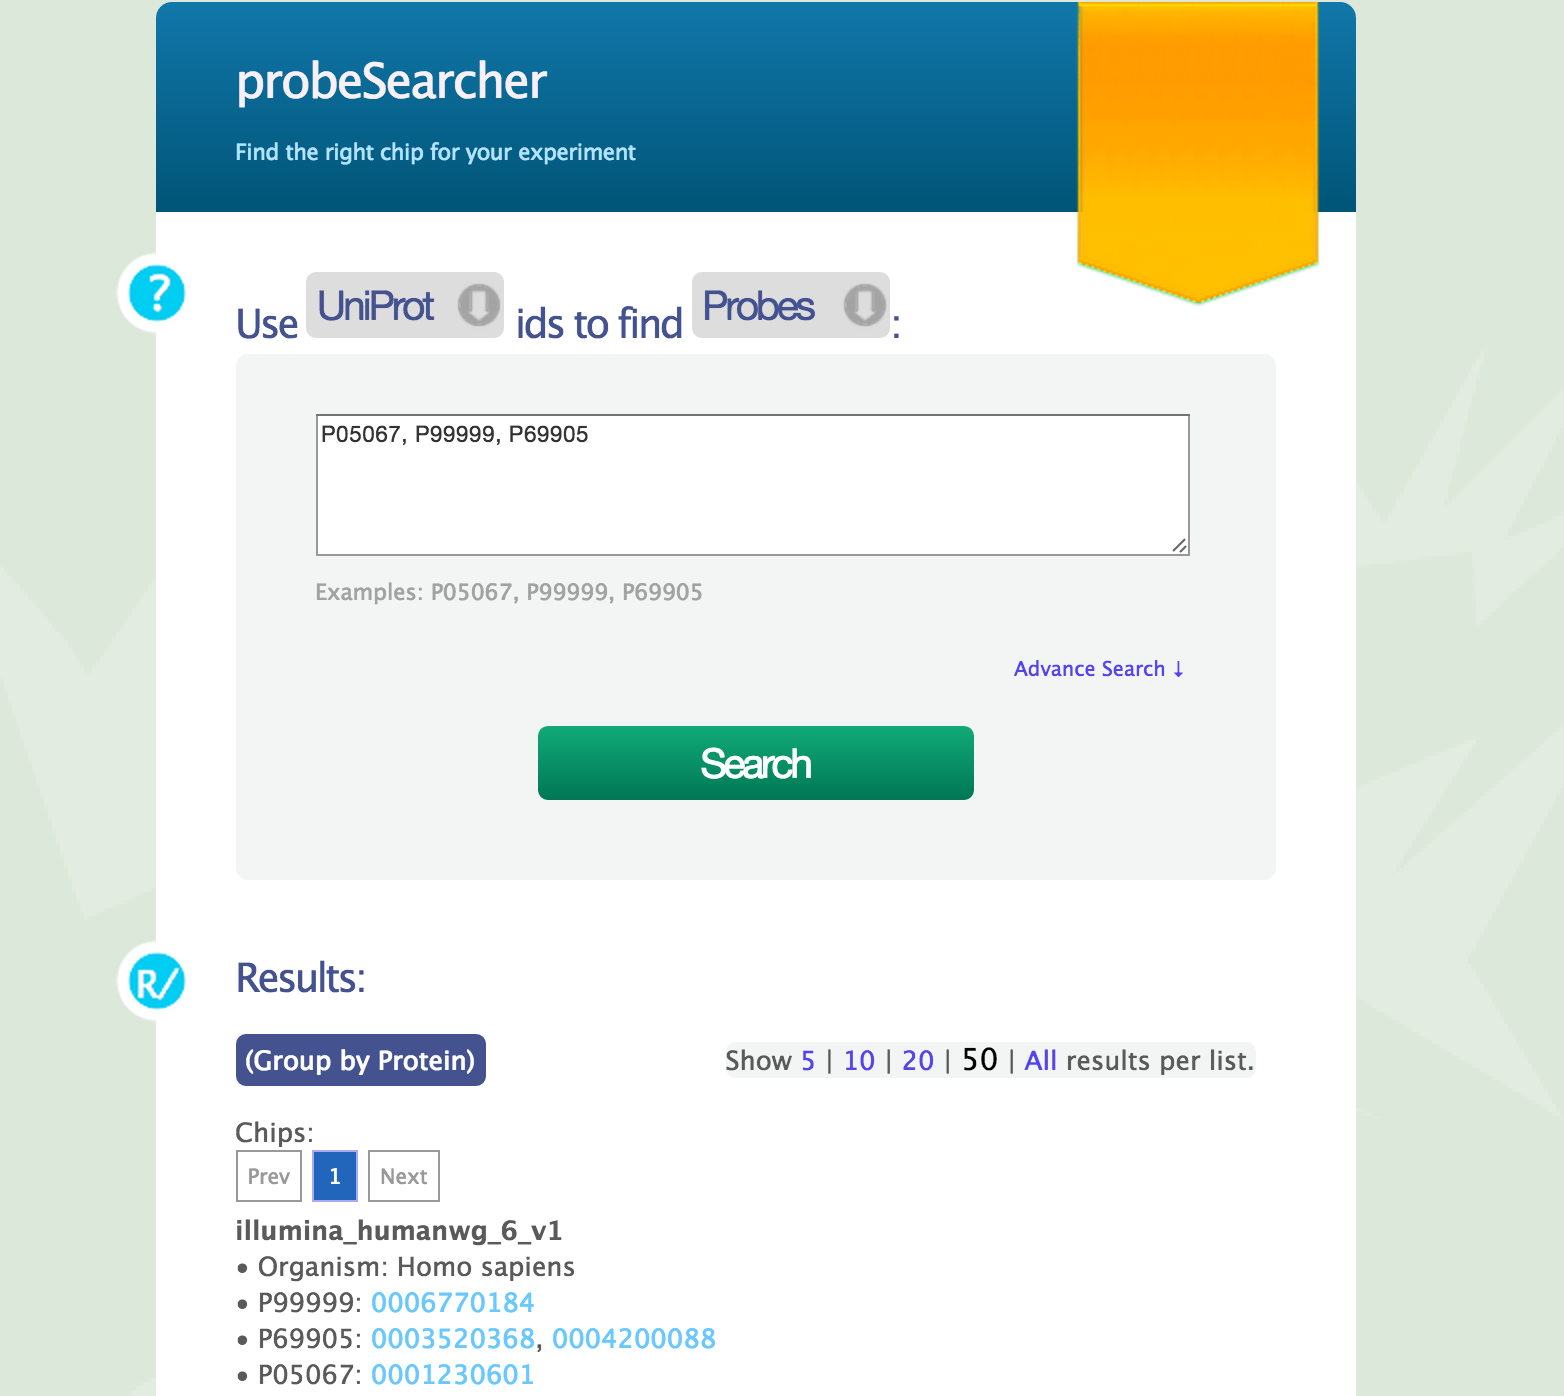
\includegraphics[width=\textwidth]{figures/probesearch.png}
\caption[Snapshot of probeSearch.]{Snapshot of probeSearch. The query includes three UniProt accession numbers: P05067, P99999, P69905. The result has been grouped by chip, and the first hit is shown at the bottom.
\label{fig:probesearch}}
\end{figure}

ProbeSearcher has a minimalistic interface (see figure \ref{fig:probesearch}), where the user is only required to input the accession numbers of interest. The default search assumes the user has UniProt IDs and is looking for the probes and ultimately the chips that include them. The search can be modified to use Ensembl IDs or inversely to find out which genes or proteins are associated with a given probe ID. The tool also offers some advanced search options, which allows the user to filter the search through different vendors and/or the target organism. 

The result of a search with probeSearch is a list of the probes linked with each of the proteins queried, including a link to the Ensembl browser where the location of the probe is shown in the context of the chromosome that contains the target sequence.

Results can also be grouped by chip, which is especially useful in the case where the query consists of several proteins, because in this way it is possible to see which proteins are represented on the same chip. For example, it is evident from the results shown at the bottom of the figure \ref{fig:probesearch}, that the chip \emph{illumina\_humanwg\_6\_v1} contains probes associated with the three protein of interest.
 
\subsubsection{Implementation Details}
We have used DAS in order to support the functionalities of probeSearcher, creating two datasources in MyDas to store and share the connections between: (i)   UniProt IDs and probes (uniprot2probes); and (ii) Ensembl IDs and probes (ensembl2probes). Using DAS for the development of this tool not only gives us the advantage of reusing robust software for the client-server communication, but also converts the data into a sharable format that can be used in other tools. For example the uniprot2probes data source can be added as another source into Dasty3 in order to include the list of related probes from several platforms.

The data stored in these sources are taken from the Ensembl BioMart \cite{KIN2011}. We have developed biomartProbes, a command line tool in java that queries BioMart, creates temporary files with the info, and uses those files to load the information into a Solr server. The DAS sources dynamically query the Solr server whenever a request is received. The source code of biomartProbes together with a packaged version can be found at \url{https://github.com/4ndr01d3/biomartProbes}.

The client of this system is a web application available in \url{http://biosual.cbio.uct.ac.za/probes-search/}. It has been written in Javascript, HTML and CSS, and takes advantage of the features provided by AJAX (described in \ref{section:dasty}). The code of this web-client can be obtained at \url{https://github.com/4ndr01d3/probeSearcher}.

\subsubsection{DAS extension for advanced search}
While developing the advanced search functionality of probeSearcher, we identified limitations in the way that DAS filters the responses of the queries triggered by the \emph{features} command. DAS queries are carried out by the \emph{features} command, which allows the querying  of annotations within  a segment. The user should input the segment ID  and optionally a range of coordinates and the server responds with the features that match the parameters. The response can be filtered by \emph{type ID} or \emph{category ID}, however this requires that the user knows all these IDs, and therefore text-based searches are not supported.

For this reason we proposed a new extension to the DAS protocol (\url{http://www.biodas.org/wiki/DAS1.6E#DAS\_search}) that adds the optional argument \emph{query} to the \emph{features} command. The content of the new command uses a syntax based on the Lucene query language, and allows the filtering of the results using the elements and arguments of DASGFF files.

The strategy behind the DAS advanced search extension was inspired by the methods used in PSICQUIC (Section \ref{subsec:psicquic}), where a similar query language called MIQL was defined in order to support advanced search options to servers containing molecular interaction data. The Lucene query language (\url{http://lucene.apache.org/core/2_9_4/queryparsersyntax.html}) and sublanguages based on it, such as MIQL or the one used in probeSeacher, were created in order to facilitate the exploration of data in indexed files, where all the information is stored in data structures that can be seen as a single table with many columns (Fields) and rows (Documents). 

Listed below are some of the most useful features of the syntax of the Lucene query language. 
\begin{itemize}
\setlength\itemsep{-0.3em}
 \item Text values are represented in between quotes and called phrases, and a phrase is composed of several terms, all of which are single words.
 \item A query can be defined by indicating which value is required in which field, using the notation of the name of the field followed by colon `:' and then the value. e.g. \emph{uniprotID:"P05067"}.
 \item Multiple queries can be combined with boolean operators: AND, OR and NOT
 \item Wildcards can be used within single terms. `?' represents any single character in that position, and `*' for multiple characters. e.g. \emph{uniprotID:"P*9"} looks for documents where the value of the field uniprotID can be of any length but should start with P and finish in 9.
\end{itemize}

The specification in \url{http://www.biodas.org/wiki/DAS1.6E#DAS\_search} contains details on the fields defined for the DAS advanced search, and the way it should be used in the \emph{features} command.

We have implemented the new extension in MyDas, including the Lucene engine as a dependency. The support for an extra command called \emph{indexer} was added to MyDas, which should be used to start the processing of any datasource, creating Lucene indexes in order to be able to give quick responses when the \emph{query} argument is used. The code of this extension is included in the MyDas repository \url{https://code.google.com/p/mydas/}.

\section{Discussion}
DAS has proven to be a successful method to publish, share and integrate data, for example, its registry reported more than 1500 data sources by the end of 2014, including important providers such as the Ensembl project and the UniProt Consortium. Several providers implemented the protocol within their own tools, in order to include third party data in the context of their own. We consider that our contributions to the different projects described in this chapter were significant to the growth of DAS, but most importantly they can improve the daily routine of scientists.

MyDas currently forms the basis for high volume DAS servers like UniProt and InterPro. It combines performance and stability with ease of installation, operation, and extension. While the easyDAS server provides a platform for DAS-based sharing of small sets of nucleic acid or protein annotations, and ProServer addresses Perl-based environments, MyDas offers a developer-friendly solution for laboratories and institutions that wish to share medium to large scale datasets in a Java-based environment. It completes the landscape of modern, open source DAS servers available to organisations sharing biomolecular data via the distributed DAS protocol. 

The writeback specification is now an official extension in DAS and is considered to be a part of the core protocol. The developed software has been well received by the community and the server implementation is now part of the official development of MyDas. In addition, the client is included in the set of plugins of DASty3, which is a widely used DAS client. Despite this, the success or failure of any collaborative system is recognised through the interaction of real users with the system, and additional time is required to determine this. We hope this system will contribute to the creation of a more publicly accessible, easily updatable, and reliable protein knowledge base.

DASty has evolved during its 10 years of existence, from a Flash widget that was highly attached to the UniProt DAS server and had a limited set of options, to a very modular and extensible framework. DASty3 is developed with modern web technologies, and has a plugin-based architecture that can be operated as an application on its own or embedded in existing websites.

Lastly, the probeSearcher tool presents a visually appealing solution to the problem of finding the available microarray chips that contain probes associated with a gene or protein of interest. This project exemplifies the potential of the DAS protocol to integrate data from different domains.

Unfortunately the DAS technology has lost momentum in recent years and the community meeting that used to take place annually hasn't occurred since February 2012. Since then, the pace of adoption of the technology has been significantly reduced. 

In August 2014, the EBI released an announcement about the retirement of the DAS services supported by the institution: \url{http://www.ebi.ac.uk/about/news/service-news/das-services-to-retire}. The justification behind this decision was the low level of usage of the services and the cost required for support and maintenance. It is also mentioned in the article that many of the EBI resources are currently supporting alternative data integration technologies. The support of some of the DAS services will be maintained by the institution until the end of 2015.

A shorter announcement was also included on the web site of the DAS registry: \url{http://www.dasregistry.org/}, indicating that the registry website will be discontinued on the 1st May 2015. We could not find any statements regarding the support of DAS services  on either the Sanger Institute's webpage or that of the Ensembl project.

It is our opinion that the DAS protocol goes further than isolated REST services, particularly on the standardisation of queries and responses. This is by no means a criticism about the release of new REST services. For example, the potential of the recently released UniProt programatic access (\url{http://www.uniprot.org/help/programmatic_access}) is undeniable, and its functionality goes further than what a regular DAS source can offer. However, the lack of a query language and response format that is common to other services forces the user to develop extra components to support each particular implementation of REST services.

We consider that withdrawing the support to DAS technology by these institutions is a step backwards for the integration of bioinformatics data, especially when it is not clear if there is a common strategy for publishing and sharing data for the services that have decided to move away from DAS. Also, we believe that the development of programmatic access in some of the providers should not be seen as a replacement of the services offered by DAS, because no matter how powerful a single one of those services is, it won't be able to include the combined data that can be aggregated by including all the data sources.
